\documentclass[a4paper,10pt]{scrartcl}
\usepackage{fullpage}
\usepackage[T1]{fontenc}
\usepackage[utf8]{inputenc}
\usepackage[ngerman]{babel}
\usepackage{amsmath}
\usepackage{amsfonts}
\usepackage{graphicx}
\usepackage{hyperref}

% neue Absatz wird mit Leerzeile begonnen:
\parindent 0pt
\parskip 12pt

\title{\textit{Höhere Algorithmitk}\\ 5. Übung}
\author{Julian Dobmann, Nico von Geyso}

\begin{document}

\maketitle

\section{Karazuba Algorithmus}

\subsection{interaktive Variante}

Aufgabe war die Implementierung des Karazuba-Algorithmus für beliebig lange
positive Binärzahlen. In unserer Implementation \texttt{Karazuba.java} führen
wir die Rekursion bis zu dem Punkt aus, bis diese mit dem nativen Datentyp
\textit{int} (32 bit) berechnet werden kann (Variante b). Das Program kann
mittels beigefügter Jar-Datei ausgeführt werden:

\begin{verbatim}$ java -jar Multiplikation.jar
Bitte gib zwei Zahlen ein (getrennt durch Enter):
18239123912591292931293310101
1921387131277547799929284571
18239123912591292931293310101 * 1921387131277547799929284571 =
35044417971429507815415551394626667822949253851377751671\end{verbatim}

\subsection{Laufzeit}

Weiterhin sollte die mittlere Laufzeit empirisch für je 10 zufällige Zahlenpaare der
Längen $n = 1000, 2000, 3000, ... 10000$ ermittelt werden. Hierzu wird für jedes
n für jedes Zahlenpaar die Laufzeit bestimmt und der Durchschnitt berechnet.
Mittels Anpassen der Parameter folgender Gleichung $T = Cn^\alpha$ sollte dann
die Laufzeit bestimmt werden.

Für unsere Implementierung scheinen $C=0.000085$ und $\alpha=2$ gut
übereinzustimmen:

$$\rightarrow T = 0.000085 n^2$$

\newpage

% generated with
% gnuplot -e "t(n) = 0.000085*n**2;plot [n=0:10000] 'karazuba.dat' with linespoints ls 3, t(n); pause 15"
\begin{figure}[ht!]
  \centering
  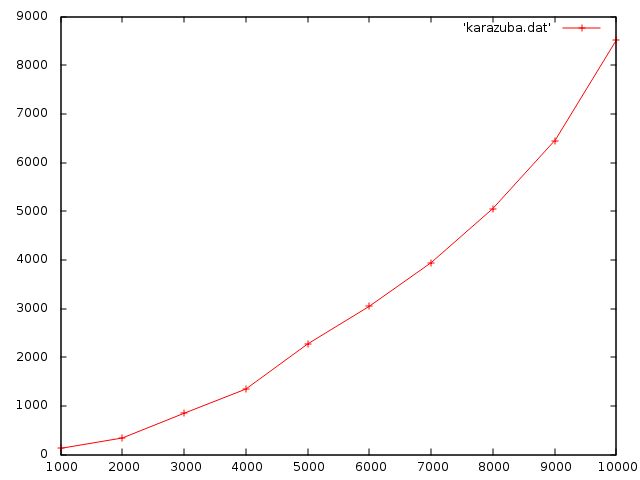
\includegraphics[width=0.6\textwidth]{plot.png}
  \caption{Plot der Laufzeiten}
\end{figure}

Die Berechnung kann mittels folgendem Parameter gestartet werden:

\begin{verbatim}$ java -jar Multiplikation.jar test\end{verbatim}

\end{document}
